

%!TEX root = ../Notes.tex
\section{Topologies} We haven't actually defined what a topology is yet. Let's fix that.
\begin{definition}
	Let $X$ be a set and $F$ be some collection of subsets of $X$ such that
	
	$1)$ $X,\emptyset \in F$.
	
	$2)$ If $U,V \in F$ then $U\cap V \in F$ .
	
	$3)$ If for all $i\in I$, $U_{i} \in F$, then $\bigcup U_{i} \in F$.
	
	Then we say that $(X,F)$ is a {\bf topological space} with {\bf open sets} the elements of $F$. We also say $F$ is the {\bf topology} on $X$. 
\end{definition}
\begin{example}
	Let $(M,d)$ be a metric space and $F$ be the set of open sets in $M$. Then $(M,F)$ is a topological space. 
\end{example}
\begin{definition}
	Let $M$ be a set and $d$ be the discrete metric, then we say $(M,F)$ is the {\bf discrete topology}. 
\end{definition}
\begin{definition}
	Let $X$ be a set with at least 2 points. Let $F=\{X,\emptyset\}$. Then we say $(X,F)$ is the {\bf indiscrete}, or {\bf concrete} topology. 
\end{definition}
\begin{definition}
	If $F_{1}$ and $F_{2}$ are topologies on $X$ and $F_{1}\subseteq F_{2}$ then we say that $F_{1}$ is {\bf weaker} than $F_{2}$, or $F_{2}$ is {\bf stronger} than $F_{1}$. 
\end{definition}

Two notes: 
\begin{itemize}
	\item weaker = fewer = coarser and stronger = more = finer. 
	\item The discrete topology is the strongest topology on $M$ and the indiscrete topology is the weakest topology on $X$. 
\end{itemize}
\begin{example}
	Let $X=R$ and $U\in F$ iff $U$ is the union of sets of the form $[a,b)$ such that $a,b\in \mathbb{R}$. (This is called the {\bf half-open interval topology}). 
\end{example}

Is this weaker, stronger, or neither compared to the usual topology?

If the interval $(a,b) \in F$, then $F$ is stronger. Let $a,b \in \mathbb{R}$, and $a<b$. Then, $(a,b)=\bigcup_{n\in \mathbb{N}}[a+\frac{1}{n},b)$, so $F$ is stronger.
\begin{example}
	Let $X=\mathbb{R}^{2}$ have the "dictionary order". This means that $(a,b)<(c,d)$ if either $a<c$ or a=c and $b<d$. 
\end{example}

Note that $U\in F$ iff $U$ is a union of ``open intervals", i.e. $\{(x,y)\ |\ (a,b)<(x,y)<(c,d)\}$.
\begin{itemize}
	\item Is a vertical line open? Yes. 
	\item Is a horizontal line open? No. 
	\item Is this topology finer or coarser than the usual topology on $\mathbb{R}^{2}$?
	
	Well, any point in a ball in the usual topology can be found in a ball of the dictionary topology, which is contained in the usual ball. Open balls are open in the dictionary topology, so the dictionary topology is finer than the usual topology. 
\end{itemize}

Note: In $\mathbb{R}$, $\bigcup_{n\in \mathbb{z}}(n,n+1)$ is open.

\mbox{ }

$Question$: Are the topologies on a set linearly ordered? No! 
\begin{example}
	Consider $\R$ with the usual topology and $(\R, F)$ with $F = \left\{ \R, \phi,47 \right\}$. We say these two topologies are {\bf incomparable}. 
\end{example}
\begin{example}
	Consider $(\mathbb{R},F)$ Define $U \in F$ if and only if either $U=\phi$ or $U=\mathbb{R}$, or $\mathbb{R}-U$ is finite. We see that if $U$ is open in $(\mathbb{R},F)$, then U is open in the usual topology. Therefore the usual topology is finer. This topology is called the {\bf finite complement topology on $\mathbb{R}$}. 
\end{example}
\begin{definition}
	A set $C$ in a topological space $(X,F)$ is {\bf closed} iff its complement $X\setminus C$ is open. 
\end{definition}

Note that a set can be both open and closed as well as neither open nor closed. (It is not a door!)
\begin{example}
	Let us consider $\mathbb{R}$ with the half-open interval topology. Then $[ 0,\infty) =\bigcup _{n \in \N} [0,n)$ is open. On the other hand, the complement of this set is $(-\infty,0) =\bigcup_{n \in\N } [-n,0)$, which is also open. Thus this is a {\bf clopen} set. 
\end{example}
\begin{example}
	A ``vertical line" in $\mathbb{R}^{2}$ with the dictionary order is both open and closed. The proof is left as exercise. 
\end{example}
\begin{lemma}
	Let $(X,F)$ be a topological space and $A$ be the set of all closed sets in X. Then: 
	\begin{enumerate}
		\item $X,\phi \in A$ 
		\item If $C,D \in A$, then $C \bigcap D \in A$ 
		\item If $C_i \in A$ for every $i \in I$, then $\bigcap_{i\in I}C_i \in A$ 
	\end{enumerate}
\end{lemma}
The proof is basically the same as that for open sets back in section 4.
\begin{definition}
	Let $(X,F)$ be a topological space and $A \subseteq X$. Let $\{ U_j\ |\ j \in J \}$ be the set of all open sets contained in $A$. Then we define $\interior{A} = \mathrm{Int}(A) = \bigcup_{j \in J} U_j$, and we say $\interior{A}$ is the {\bf interior} of $A$. 
\end{definition}
\begin{smallfact}
	Let $(X,F)$ be a topological space and $A \subseteq X$. Then 
	\begin{enumerate}
		\item $\interior A \subseteq A$ 
		\item $\interior A$ is open 
		\item If $U\subseteq A$ is open, then $U\subseteq \interior A$ 
		\item $A$ is open iff $A = \interior A$. 
	\end{enumerate}
\end{smallfact}
\begin{proof}
	\begin{enumerate}
		\item Since $\interior A = \bigcup_{j\in J} U_j$ and $U_j \subseteq A$ for every $j \in J$, $\interior A\subseteq A$. 
		\item By definition, $\interior A$ is a union of open sets, so $\interior A$ is open. 
		\item Since $U$ is open in $A$, $U \in \{ U_j\ |\ j\in J\}$. Therefore $U\subseteq \bigcup_{j\in J} U_j = \interior A$. 
		
		Note that this means that $\interior A$ is the ``largest'' open set in $A$. 
		\item Suppose that $A = \interior A$. Then $\interior A$ is open by part (2), hence $A$ is open.
		
		Conversely, suppose that $A$ is open. Then $A\in \{U_j\ |\ j\in J\}$. Hence $A \subseteq \interior A$. From (1), $A = \interior A$. 
	\end{enumerate}
\end{proof}
\begin{example}
	In the half-open interval topology on $\R$, $\Int((0,1])=(0,1)$. To prove this, assume that $1\in \Int((0,1])$ and show that it leads to a contradiction. 
\end{example}
\begin{example}
	In the finite-complement topology on $\R$, $\Int((0,1])= \emptyset$. This follows from the fact that $\R$ is infinite and all subsets of $(0,1]$ are finite. 
\end{example}
\begin{example}
	In the dictionary-order topology on $\R^2$, $\Int( [ 0,1] \times [ 0,1] ) = [0,1] \times (0,1)$. 
	\[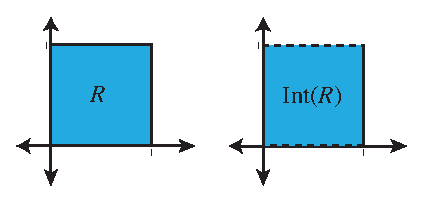
\includegraphics[width=300pt]{images/topologies/dictionary_order_interior}\]
\end{example}
\begin{definition}
	Let $A$ be a subset of a topological space $(X,F)$, and let $\{ F_j\ |\ j \in J \}$ be the set of all closed sets containing $A$. Then the {\bf closure} of $A$ is defined as $\closure{A} = cl(A) = \bigcap_{j \in J}F_j$. 
\end{definition}
\begin{smallfact}
	Small facts about closures: 
	\begin{enumerate}
		\item $A \subseteq \closure{A}$ 
		\item $\closure{A}$ is closed 
		\item If $A \subseteq C$ and $C$ is closed, then $\closure{A}\subseteq\closure{C}$ 
		\item $\closure{A}=A$ if and only if $A$ is closed. 
	\end{enumerate}
\end{smallfact}
The proofs are left as exercises.
\begin{example}
	In $\R$ with the usual topology, $\mathrm{cl}\left(\left\{ \frac{1}{n}|n \in \N \right\}\right) = \left\{\frac{1}{n}|n \in \N \right\} \cup \{ 0\}$ 
\end{example}
\begin{example}
	In $\R$ with the half-open interval topology, $\mathrm{cl}((0,1])=[ 0, 1]$ 
\end{example}
\begin{lemma}
	(an Important Lemma)\\
	Let $(X,F)$ be a topological space and $Y \subseteq X$. Then $ p \in \closure{Y}$ if and only if for every open set $U\subseteq X$ containing $p$, $U \cap Y \neq\emptyset$. 
\end{lemma}
\begin{proof}
	Let $p \in \closure{Y}$ and $U\subseteq X$ be open with $p \in U$. Suppose $U \cap Y = \emptyset$ and let $C=X\setminus U$. Then $p\notin C$ because $p \in U$. It follows that $\overline{Y} \subseteq C$ because $Y \subseteq C$ and $C$ is closed. We obtain that $p \in C$, which is a contradiction.
	
	Conversely, suppose that for every open set $U\subseteq X$ such that $p \in U$, $U\cap Y \neq \emptyset$. Let $C\subseteq X$ be closed such that $Y \subseteq C$. Suppose $p \notin C$. Let $U=X\setminus C$, which is open with $p \in U$. Now $U \cap Y \neq\emptyset$, so there exists some $x \in U \cap Y$. This means that $x\in X\setminus C$, i.e. $x \notin C$. But since $Y \subseteq C$, we have $x \notin Y$, a contradiction. Therefore we conclude that $p \in \closure{Y}$. 
\end{proof}
\begin{corollary}
	Suppose that $U$ is an open set in a topological space $(X,F)$ and $Y \subseteq X$. If $U \bigcap \closure{Y}\neq\emptyset$, then $U \bigcap Y \neq \emptyset$. 
\end{corollary}

\proof The proof is immediate from the important lemma.

Now we can use the important lemma to prove that in $\R$ in the usual topology, $\mathrm{cl}(\{1/n\ |\ n\in\N\}) = \{1/n\ |\ n\in\N\}\cup\{0\}$. Here, we can show that for all open sets $U$ containing 0, $U \bigcap\left\{ \frac{1}{n}\ |\ n \in \mathbb{N} \right\} \neq \emptyset$.
